\documentclass{sig-alternate}
\usepackage{graphicx}
\usepackage[usenames,dvipsnames]{color}

\newcommand{\gd}[1]{\textcolor{ForestGreen}{GD: #1}}

\begin{document}
%
% --\item Author Metadata here ---
\conferenceinfo{WWW}{'15}
%\CopyrightYear{2007} % Allows default copyright year (20XX) to be over-ridden \item IF NEED BE.
%\crdata{0-12345-67-8/90/01}  % Allows default copyright data (0-89791-88-6/97/05) to be over-ridden \item IF NEED BE.
% --\item End of Author Metadata ---

% \title{The Evolution of Micro-task Crowdsourcing Markets}
\title{The Market for HITs: Throughput Uncertainty and the Market Mechanism}
\subtitle{The Case of Amazon MTurk}
% The Evolution of Micro-Task Crowdsourcing Markets —- The Case of Amazon Mechanical Turk
% The Dynamics of Micro-Task Crowdsourcing -- The Case of Amazon MTurk
% Anatomy of a Micro-Task Crowdsourcing Platform
% Unravelling Micro-Task Crowdsourcing Dynamics/Processes
% The Market for HITs: Throughput Uncertainty and the Market Mechanism


%\numberofauthors{1}
\author{Djellel E. Difallah, Michele Catasta, Gianluca Demartini, Panagiotis G. Ipeirotis, Philippe Cudr\'e-Mauroux}

\maketitle
\begin{abstract}
Micro-task crowdsourcing is rapidly gaining popularity among research communities and businesses as a means to leverage Human Computation in their daily operations. Unlike any other ``technology'', a crowdsourcing platform is subject to human factors that affect its performance, both in terms of speed and quality. Indeed, such factors shape the \emph{dynamics} of the crowdsourcing market. For example, a known behavior of such markets is that increasing the reward of a task would lead to faster results. However, it is still unclear how different dimensions interact each other: reward, task type, market competition, requester reputation, etc.

In this paper we adopt a data-driven approach to perform a long-term analysis of a popular micro-task crowdsourcing platform to understand behavior evolution of its main actors: workers, requesters, tasks, and platform. We leverage the main findings of our five year log analysis to generate features used in a predictive model for the expected performance of a batch of tasks published on the crowdsourcing platform at a specific point in time by a certain requester.
\end{abstract}

% A category with the (minimum) three required fields
\category{H.4}{Information Systems Applications}{Miscellaneous}
%A category including the fourth, optional field follows...
% \category{D.2.8}{Software Engineering}{Metrics}[complexity measures, performance measures]

\terms{Design, Experimentation, Human Factors}

\keywords{Crowdsourcing, social networks, log analysis}

%!TEX root = ../dynamics.tex
\section{Introduction}\label{sec:intro}
The micro-task crowdsourcing market has seen a rapid growth in the last five years. This is correlated with the fact that more data is available to enterprises and that data is an asset within business processes. While data is available, its quality is not always high and manual processing is often necessary. To this end, outsourcing  data processing tasks  like image tagging, audio transcription, translation, etc. to a large crowd of individuals has become popular.

%micro-task Crowdsourcing platform
To perform such Human Intelligence Tasks (HITs) crowdsourcing platforms have been developed. Such platforms serve as place where the crowd (i.e., people willing to perform small tasks in exchange of a small monetary reward, also know as \emph{workers}) and work providers (i.e., also known as \emph{requesters}) meet. \gd{describe crowdsourcing process of publishing tasks, completing task, getting results, rewarding}

%
In this paper we analyze the evolution of a very popular micro-task crowdsourcing platform over the last five years and propose techniques to support requesters in posting HITs to the market in an effective way. Using features derived from a large-scale analysis of platform logs, we propose methods to predict the throughput of the crowdsourcing platform for a batch of HITs published by a certain requester at a certain point in time. This prediction is based on different features including current platform load, requester reputation, popular task types, etc.

\gd{summarize main findings}


In summary, the main contributions of this paper are:
\begin{itemize}

	\item An analysis of the evolution of a popular micro-task crowdsourcing market looking at dimensions like topics, task types, reward, worker location.

	\item A large-scale classification of 2.5M HITs published on Amazon MTurk.

	\item An effective model to predict the completion speed of a batch published on Amazon MTurk at a certain point by a certain requester.

	\item An online service with evolution statistics and services for requesters to better design their HIT metadata (e.g., keywords, reward, etc.)

\end{itemize}


The rest of the paper is structured as follows.
In Section \ref{sec:relwork} we overview recent work on micro-task crowdsourcing specifically focusing on works improving efficiency of crowdsourcing systems.
%!TEX root = ../dynamics.tex
\section{Related Work}\label{sec:relwork}

\subsection{Micro-task Crowdsourcing}

A very popular platform is Amazon MTurk\footnote{\url{http://mturk.com}} which provides access to a crowd of workers distributed worldwide but mainly composed of people based in USA and India \cite{mturk}.

Workers share experiences about HITs and requesters within web forums and ad-hoc websites \cite{turkopticon}. Such requester `reviews' serve as a way to measure requester reputation which is assumed to be a reason for obtaining answers efficiently from the crowd \cite{}. In this work we experimentally show the effect of platform and requester properties on crowd efficiency.  \gd{rephrase last sentence?}


\subsection{Human Computation}
Micro-task crowdsourcing is used to improve the quality of purely machine-based systems in order to combine both the scalability of machines over large amounts of data as well as the quality of human intelligence to process and understand data.
Many examples of such hybrid approaches exist.
Crowd-powered databases \cite{crowddb} leverage crowdsourcing to deal with incomplete data, complex data integration problems, graph search, and joins \cite{crowder,graphsearch,crowdjoins}.
Semantic Web systems leverage the crowd for schema matching \cite{crowdmap}, entity linking \cite{zencrowd}, and ontology engineering \cite{bioonto}.
Information Retrieval systems use crowdsourcing for evaluation purposes \cite{mizzaroalonso}.

When building systems that build on top of crowdsourcing platforms, two main challenges have to be dealt with: effectiveness and efficiency  of the crowd.

\subsection{Crowdsourcing Effectiveness}

A very important dimension for crowdsourcing effectiveness is \emph{answer aggregation}, that is, after assigning the same HIT to multiple workers in the crowd, effectively aggregate their answers in a final results to be output back from the crowdsourcing platform to the system leveraging human computation. Multiple approaches have been proposed for this aspect of crowdsourcing quality (e.g.,
\cite{Venanzi:2014:CBA:2566486.2567989,square,zencrowd,Hosseini:2012:ALM:2260641.2260661}).
% 
A recent approach which results in effective aggregation is \cite{Venanzi:2014:CBA:2566486.2567989} where authors detect communities of workers with similar answering patterns to re-weight their answers even when little evidence of individual worker quality is available (i.e., just few HITs have been completed).


More than aggregation, identifying the best worker in the crowd is another mean to obtain quality answers from the crowd \cite{pickacrowd,bozzon}.

More recently, \cite{Jung14-hcomp} aims at predicting work quality looking at worker activities over time.

\subsection{Crowdsourcing Efficiency}

In \cite{Kittur:2013:FCW:2441776.2441923} authors provide their view on how the crowdsourcing market should adapt specifically focusing on how to  support full-time crowd workers. On the other hand, in this work we perform a data-driven analysis of the evolution of micro-task crowdsourcing over the past five years using the findings of such analysis as features to support requesters while publishing HITs on these platforms in an effective way.

\cite{finishthem,scaleup}

To improve human computation efficiency, it is key to support worker in being more efficient while working on HITs. For example, workers spend way too much time in searching for HITs to work on \cite{Kucherbaev:2014:TET:2598153.2602249}.






% final remark
Our work is complementary to existing work as we present a data-driven study of the evolution of micro-task crowdsourcing over five years as a support evidence of the ongoing efforts to improve crowdsourcing quality and efficiency that we have described.

\section{The Amazon Mechanical Turk Crowdsourcing Platform}

\section{The Evolution of MTurk}
2009-2014
\subsection{A Data-driven Analysis}
Datasets: tracker, to, 
\paragraph{Which Topics Were Popular Over Time?}

\begin{figure}[htbp]
	\centering
		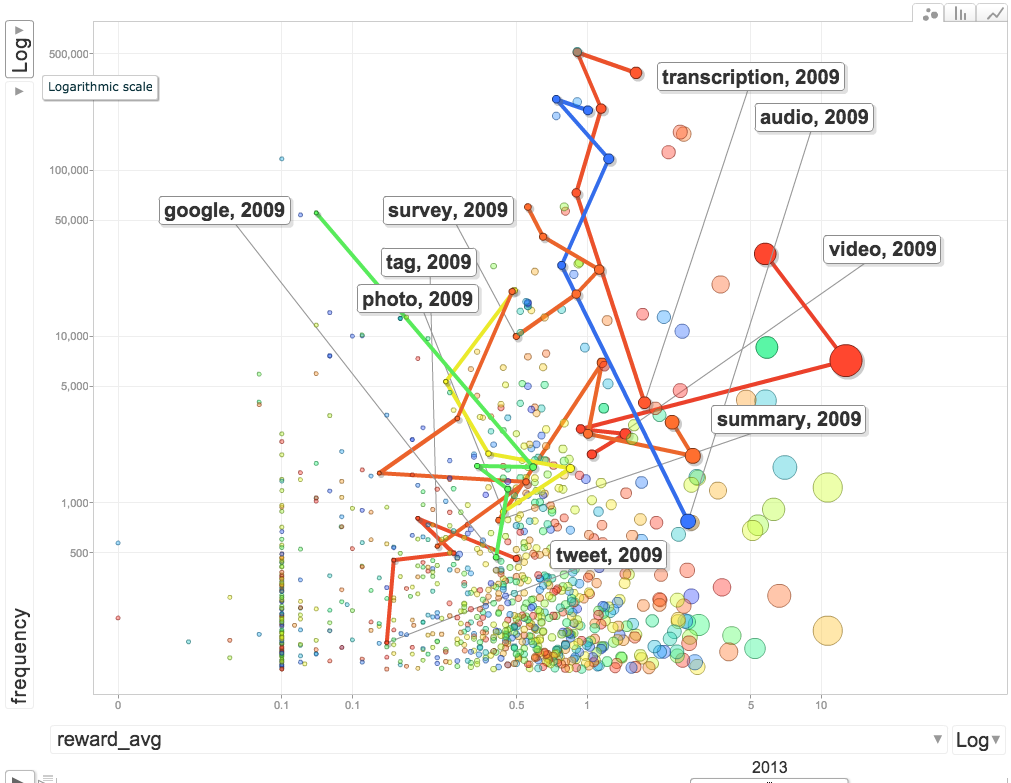
\includegraphics[width=0.5\textwidth]{tagEvolution.png}
	\caption{tagEvolution}
	\label{fig:tagEvolution}
\end{figure}

\paragraph{Which Countries Were Preferred by Requesters Over Time?}
top keywords per country (over time)
% \subsection{Why Did Certain Requesters Quit?}
% \subsection{Does reputation Improve Throughput?}


%!TEX root = ../dynamics.tex
\section{Large-Scale HIT Type Analysis}\label{sec:type}
In this section we present the results of a large-scale analysis of the evolution of HIT \emph{types} published on the \amt{} platform.
For such analysis we use the definition of HIT types proposed by \cite{Gadiraju:2014:TMW:2631775.2631819} in which authors perform an extensive study involving 1000 crowd workers to understand their working behavior. 

\subsection{A Classification of HIT Types}
Next, we describe the six top-level classes as introduced by \cite{Gadiraju:2014:TMW:2631775.2631819}.

\begin{itemize}[noitemsep,topsep=0pt,parsep=0pt,partopsep=0pt]

	\item Information Finding (IF): Searching the Web to answer a certain information need. For example, ``Find the cheapest hotel with ocean view in Monterey Bay, CA''.
	
	\item Verification and Validation (VV): Verifying certain information or confirming the validity of a piece of content. Examples include checking Twitter accounts for spamming behaviors.

	\item Interpretation and Analysis (IA): Interpreting Web content. For example, ``Categorize product pictures in a predefined set of categories'', or ``Classify the sentiment of a tweet''.
	
	\item Content Creation (CC): Generating new content. Examples include summarizing a document  or transcribing an audio recording.

	\item Surveys (SU): Answering a set of questions related to a certain topic (e.g., demographics or customer satisfaction). 
	
	\item Content Access (CA): Accessing some Web content. Examples include watching on-line videos or clicking on provided links.

\end{itemize}

\subsection{Supervised HIT Type Classification}
Using the definition of HIT types described above, we trained a supervised machine learning model to classify HIT types based on their metadata. The features we used to train a Support Vector Machine (SVM) model are: HIT title, description, keywords, reward, date, allocated time, and batch size.

% labelling setup
To train and evaluate the supervised model we created labelled data: We uniformly sampled 5000 HITs over the entire five-years dataset and manually labelled their type by means of crowdsourcing. In detail, we asked workers on MTurk to assign each HIT to one of the predefined classes by presenting them with the title, description, keywords, reward, date, allocated time, batch size for the HIT. The instructions also contained the definition and examples for each task type. Workers could label tasks as `Others' when unsure or when the HIT did not fit in any of the available options.

% labelled data
After assigning each labelling HIT to three different workers in the crowd, a consensus on the task type label was reached in $89\%$ of the cases (i.e., 551 cases with no clear majority). A consensus was reached when at least two out of three workers agreed on a HIT type label. The other cases, that is, when the workers provided different labels or when they where not sure about the HIT type have been removed from our labelled dataset.

% classification evaluation
Using the labelled dataset we trained a multi-class SVM classifier for the 6 different task types and evaluated its quality with 10-folds cross validation over the labelled dataset. Overall, the trained classifier obtained Precision of $0.895$, Recall of $0.899$, and F-Measure of $0.895$. Most of the classifier errors (i.e., 66 cases) were done by incorrectly classifying IA instances as CC.

% top features
Performing feature selection for the HIT type classification problem we observed that the best features according to information gain are the HIT allotted time and reward: This indicates that HITs of different types are associated with different levels of reward as well as different task duration (i.e., longer and better paid tasks versus shorter and paid worse). 
Most distinctive keywords for identifying HIT type are `transcribe', `audio', and `survey' which clearly identify CC and SU HITs.
 
% classification at scale
Using the classifier trained over the entire labelled dataset, we then performed a large scale classification of the type for all 2.5M HITs in our collection. This allows us to study the evolution over time of task types on the \amt{} platform which we present next.

\subsection{Task Type Popularity Over Time}
Using the result of the large-scale classification of HIT types, we  analyze which  types of HITs have been published over time.
Figure \ref{fig:cat_trends} shows the evolution of task types published on \amt{}\ .
% 
We can observe that, in general, the most popular type of task is Content Creation.
% 
In terms of observable trends, we note that, while there is a general increase of the volume of tasks of a certain type on the platform,  CA tasks have been decreasing over time. This can be explained  by the enforcement of \amt{} terms of service which state that workers should not be asked to create accounts on external website or be identified by the requester.
% 
In the last three years, SU and IA tasks have had the biggest increase.

\begin{figure}[htbp]
	\centering
		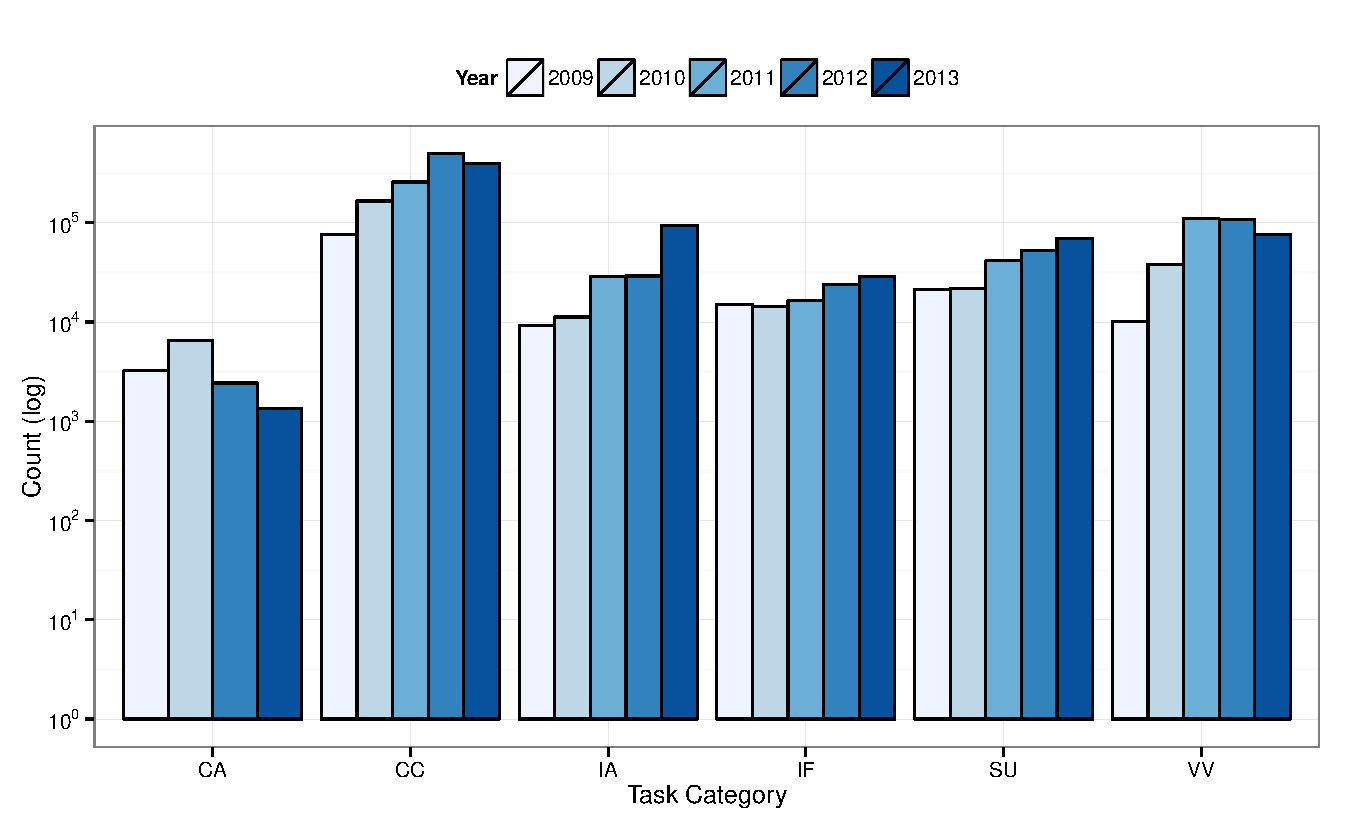
\includegraphics[width=0.5\textwidth]{figures/category_trends}
	\caption{Popularity of HIT types over time.}
	\label{fig:cat_trends}
\end{figure}


%!TEX root = ../dynamics.tex
\section{Analyzing the Features Affecting Batch Throughput}
\label{sec:throughput}
Next, we turn our attention to analyzing the factors that influence the progress (or the pace) of a batch, how those factors influence each other and how their importance changes over time. 

In order to conduct this analysis, we try to predict the throughput of a batch of tasks (or how many HITs get will get completed in the next time frame). 
The value we aim to predict is the batch \emph{throughput}, that is, the numbers of HITs that  will be completed for a given batch within the next time frame of 1 hour (i.e.,  the $DIFF\_HIT$ feature is a target class).
Specifically, we model this task as a regression problem using 29 features; some of them were used in the previous section to classify HIT type, we describe the remaining ones in Appendix A.

\subsection{Experimental Setup}

To predict the throughput of a batch at time $T$, we train a Random Forest Regression model with samples taken in the range $[T-\delta, T)$ where $\delta$ is the size of the time window that we are   considering directly prior to time $T$. The rational behind this approach is that the throughput should be directly correlated to the current and recent market situations. 
The research question we tackle in this context is:\\ \emph{``How much historical data does one need to consider to predict the throughput effectively?"}. \\ To answer this, we proceed by varying $\delta$.
To evaluate the effectiveness of $\delta$ values, we compute the coefficient of determination  $R^2$ \cite{sklearnweb, sklearn}.
In this experiment, we considered  data from June to October 2014 and hourly observations (see Section \ref{sec:tracker}), from which we uniformly sampled 50 time points for evaluation purposes. Finally, for each time point we considered a training time frame $\delta$ ranging from 1 hour to 24 hours. 

\subsection{Prediction}
In Figure \ref{fig:accuracy}, we observe that the computed evaluation score reaches its highest values when using the latest 4 hours as training time-frame, then decreases when we increase the training time-frame, to finally again increase and stabilize when we use up to 24 hours training data.
Note that the score is relatively low for batches with low throughput. 

Our prediction results (when using 4hours window) versus actual throughput values are shown in Figure \ref{fig:pred}. The prediction works best for larger batches having a large momentum as the Figure suggests.

\begin{figure}[t!]
	\centering
		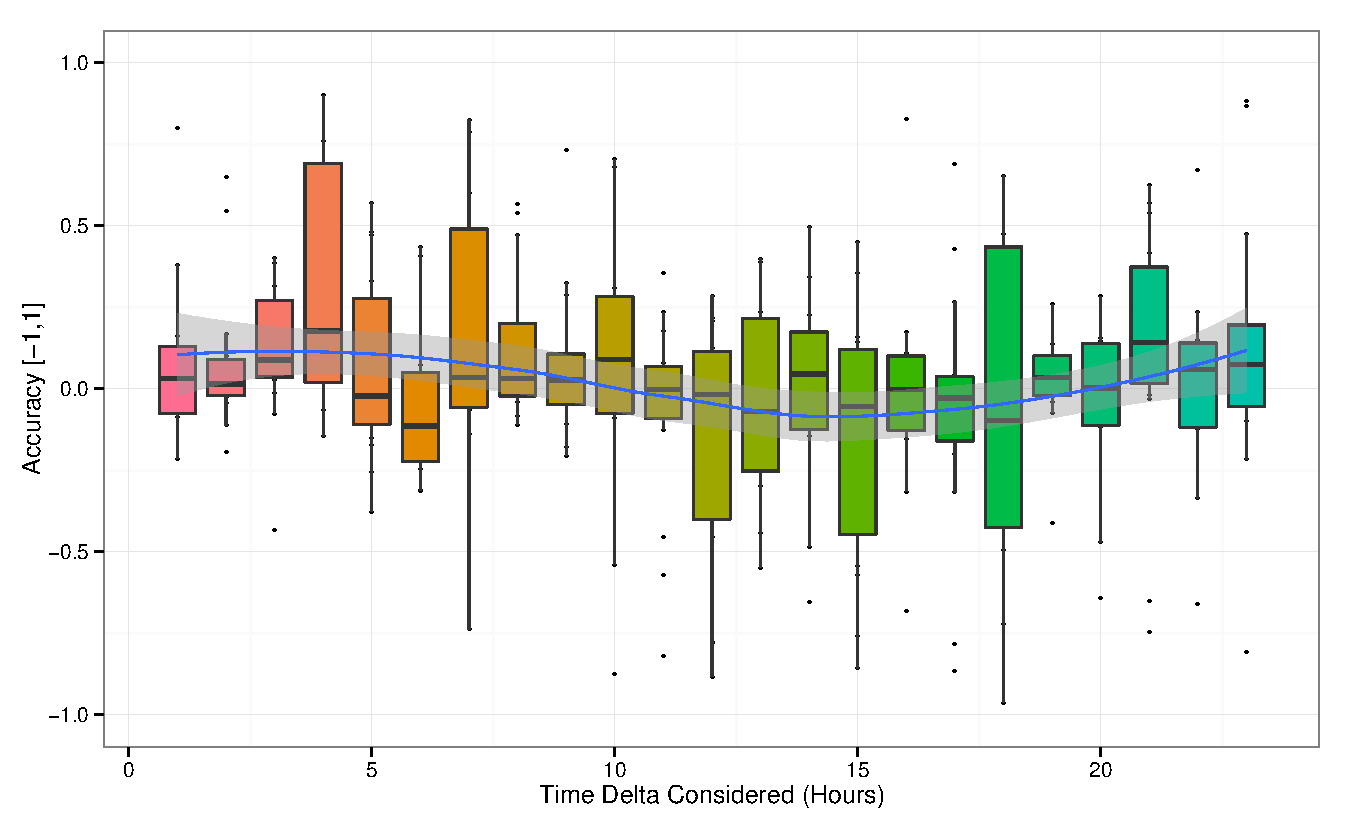
\includegraphics[width=0.48\textwidth]{figures/ML_accuracy}
	\caption{Score ($R^2$) of the throughput prediction when considering larger time spans as training sets. The red dots are average values, while the boxes represents the median, first and third quartiles. N.B., the implementation of the score function used in our experiments allows for negative values.}
	\label{fig:accuracy}
\end{figure}
\footnotetext{\url{http://scikit-learn.org/stable/modules/generated/sklearn.metrics.r2_score.html}}

\begin{figure}[t!]
	\centering
		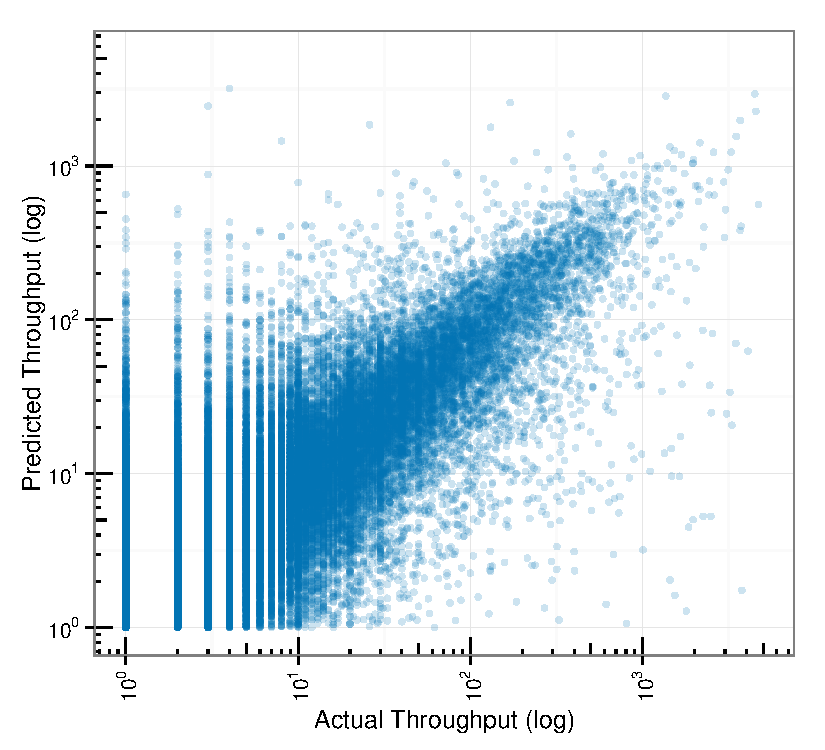
\includegraphics[width=0.48\textwidth]{figures/predictions_3}
	\caption{Prediction vs actual throughput values. Prediction is more accurate for larger throughput values. This suggests that the throughput will remain high until the batch gets smaller.}
	\label{fig:pred}
\end{figure}

\subsection{Features Importances}
In order to better grasp the characteristics of the batch throughput, we examine the prediction's features importances to understand which ones contributes more.

Figure \ref{fig:importances} shows the  contribution of the top 4 features and how it varies  when we increase the training time-frame. The rest of the features importances are listed in Table \ref{table:feats}, their slope indicates whether the feature is gaining importance overtime (positive value) or decreasing in importance (negative value).
The most important feature is $HIT\_Available$, that is, the current size of the batch. Indeed, as observed by previous work, larger batches tend to attract more workers \cite{mturk,crowddb}. This feature becomes less important when we consider longer periods, partly because of noise, but, most importantly, because of other features like $age\_minutes$ and $left\_minutes$, which encode additional facts and suggest that the crowd is sensitive to the newly posted HITs, or how \emph{fresh} the HITs are. To better understand this phenomenon, we conduct an analysis on what attracts the workforce to the the platform in the next section.

\begin{figure}[t!]
	\centering
		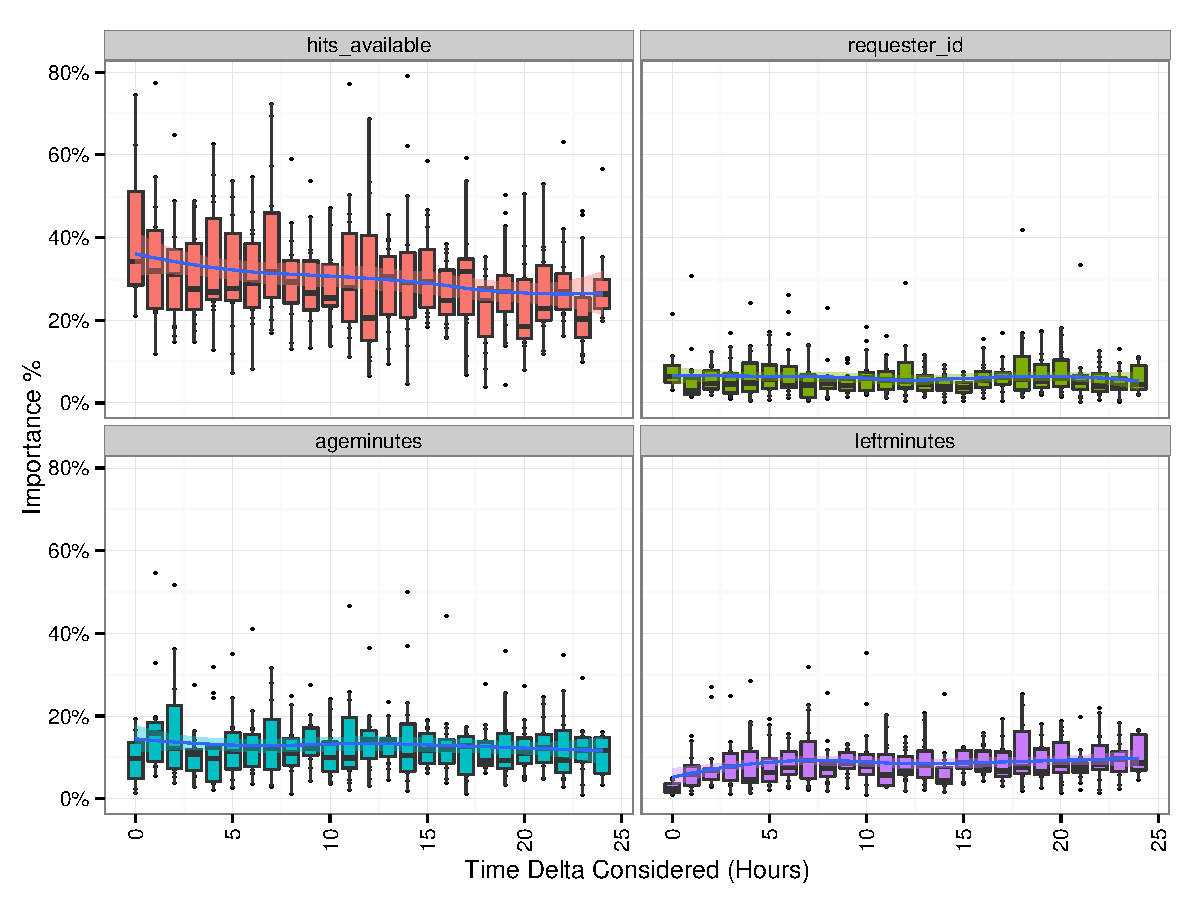
\includegraphics[width=0.5\textwidth]{figures/importances}
	\caption{Computed feature importance when considering larger training sets for the prediction.}
	\label{fig:importances}
\end{figure}


\begin{table}[t!]
\scriptsize
\begin{tabular}{|c|c|c|c|c|}
\hline
Feature              & mean      & stddev    & slope     & intercept \\
\hline
hits\_available      & 29.8606 & 13.4247 & -0.0257 & 34.4940 \\
ageminutes           & 12.9087 &  8.1967 & -0.0050 & 13.8181 \\
leftminutes          &  8.7300 &  5.5530 & 0.0061 & 7.6290 \\
requester\_id        &  6.2147 &  5.2943 & -0.0011 & 6.4305 \\
title                &  5.6441 &  4.2604 & -0.0033 & 6.2519 \\
description          &  4.8823 &  3.8975 & -0.0065 & 6.0617 \\
keywords             &  4.3765 &  3.3860 & -0.0074 & 5.7095 \\
time\_alloted        &  3.7994 &  3.6820 & -0.0010 & 3.9965 \\
reward               &  3.5439 &  2.7426 & -0.0011 & 3.7458 \\
totalapproved        &  2.5259 &  3.5108 & 0.0033 & 1.9311 \\
tasktype             &  2.1370 &  2.2673 & -0.0008 & 2.2986 \\
start\_time          &  1.2257 &  1.4123 & 0.0049 & 0.3325 \\
hitsAvailableUI      &  1.1428 &  1.2062 & 0.0039 & 0.4380 \\
diffHitsUI           &  1.0557 &  1.1237 & 0.0038 & 0.3568 \\
hitGroupsAvailableUI &  1.0438 &  1.0219 & 0.0034 & 0.4169 \\
diffGroupsUI         &  1.0408 &  1.0658 & 0.0030 & 0.4835 \\
master               &  0.9943 &  2.3816 & -0.0012 & 1.2134 \\
diffGroups           &  0.9660 &  0.9349 & 0.0032 & 0.3863 \\
rewardsArrived       &  0.9543 &  1.0710 & 0.0032 & 0.3698 \\
hitsCompleted        &  0.9293 &  0.9453 & 0.0031 & 0.3593 \\
percHitsCompleted    &  0.8974 &  0.8548 & 0.0030 & 0.3543 \\
location             &  0.8957 &  1.7592 & 0.0004 & 0.8184 \\
diffRewards          &  0.8920 &  0.8967 & 0.0023 & 0.4622 \\
rewardsCompleted     &  0.8890 &  0.8896 & 0.0026 & 0.4056 \\
percHitsPosted       &  0.8462 &  0.9552 & 0.0021 & 0.4618 \\
diffHits             &  0.8462 &  0.7514 & 0.0024 & 0.3972 \\
hitsArrived          &  0.7562 &  0.7946 & 0.0021 & 0.3760 \\
approvalrate         &  0.0000 &  0.0000 & 0 & 0 \\
\hline
\end{tabular}
\caption {Importances of the features used in the prediction experiment. A large mean indicates a better overall contribution to the prediction. A positive slope indicates that the feature is gaining in importance when the considered time window increases.}
\label{table:feats}
\end{table}

\section{Conclusions}

\bibliographystyle{abbrv}
\bibliography{crowd}

\end{document}
